\section{Incorporating MINERvA components into ProtoDUNE-ND}
\label{sec:MINERvA}
The MINERvA experiment~\cite{minerva-nim} is located in the MINOS ND hall in which ProtoDUNE-ND will be installed, and is due to complete its data-taking in spring--summer 2019. The collaboration is currently considering its detector decommissioning plan, and it has been suggested that some components of the MINERvA tracking scintillator detector could be repurposed for ProtoDUNE-ND. As discussed in Section~\ref{sec:protodune-nd}, all DUNE ND designs considered in Ref.~\cite{dune_ndcsg} include some fast scintillator component. In this section, we outline the possible uses of the MINERvA detector components, and consider potential detector physics studies that they would bring to ProtoDUNE-ND.

\subsection{Description of the MINERvA detector}

\begin{figure}[htb]
  \centering
  \subfloat[Front view] {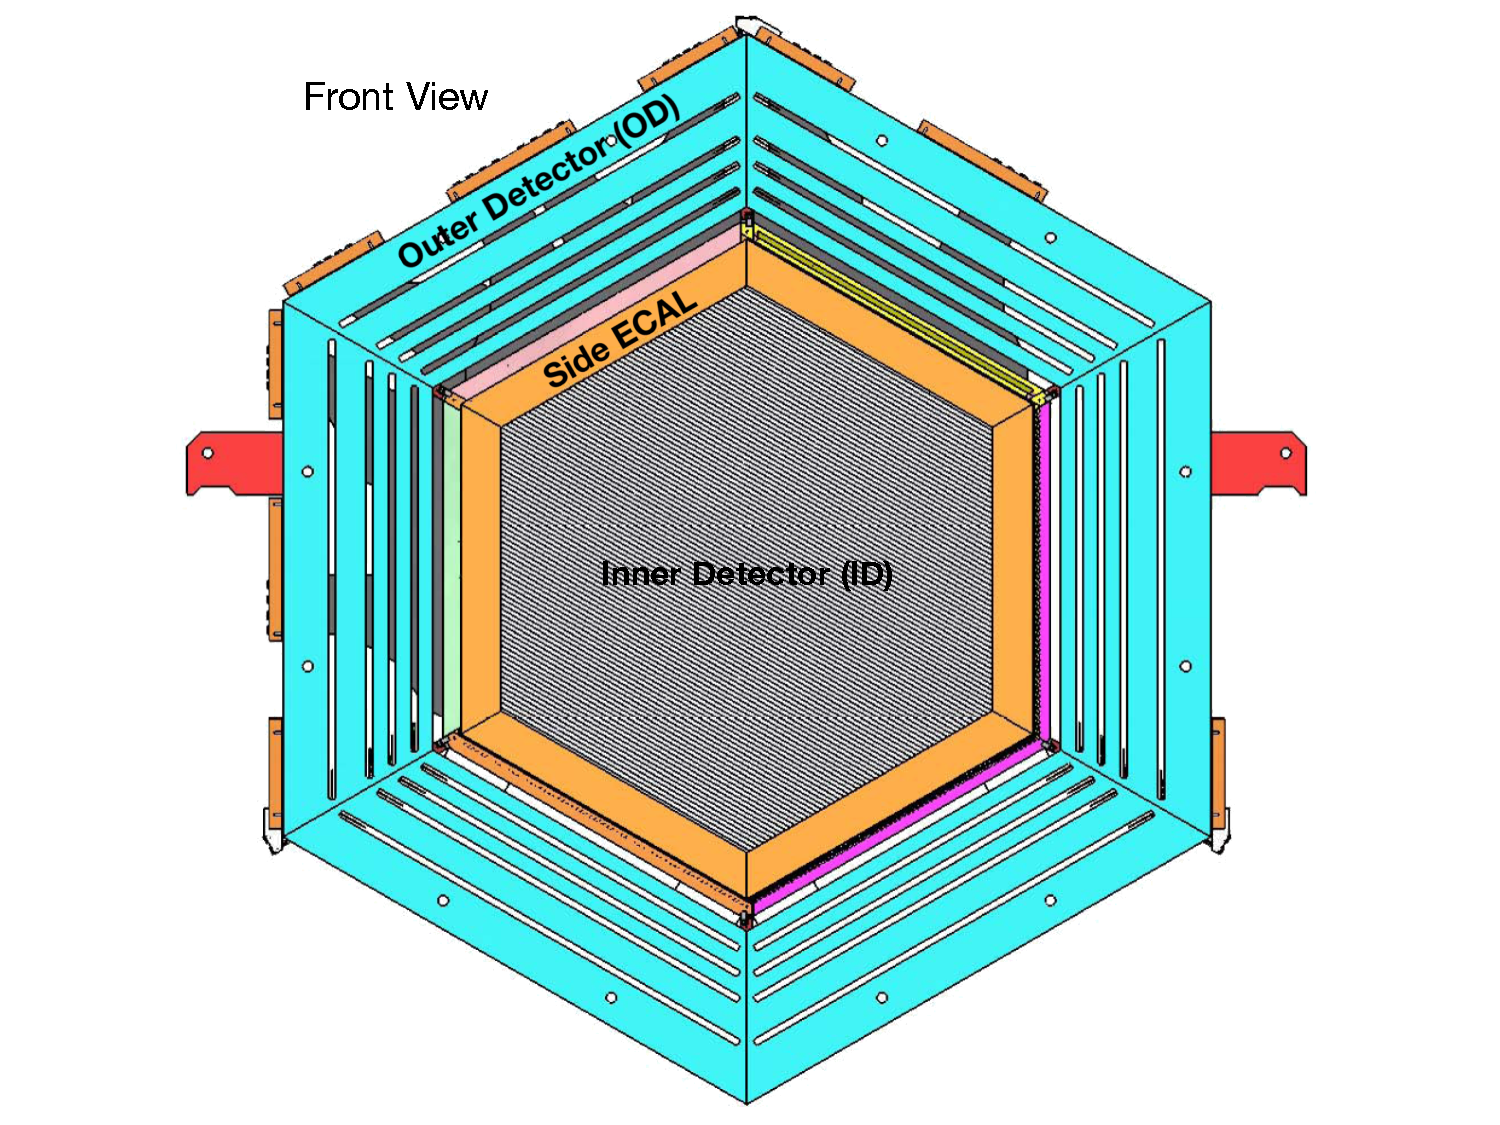
\includegraphics[width=0.35\textwidth]{plots/minerva_module_transverse.pdf}}
  \subfloat[Side view]  {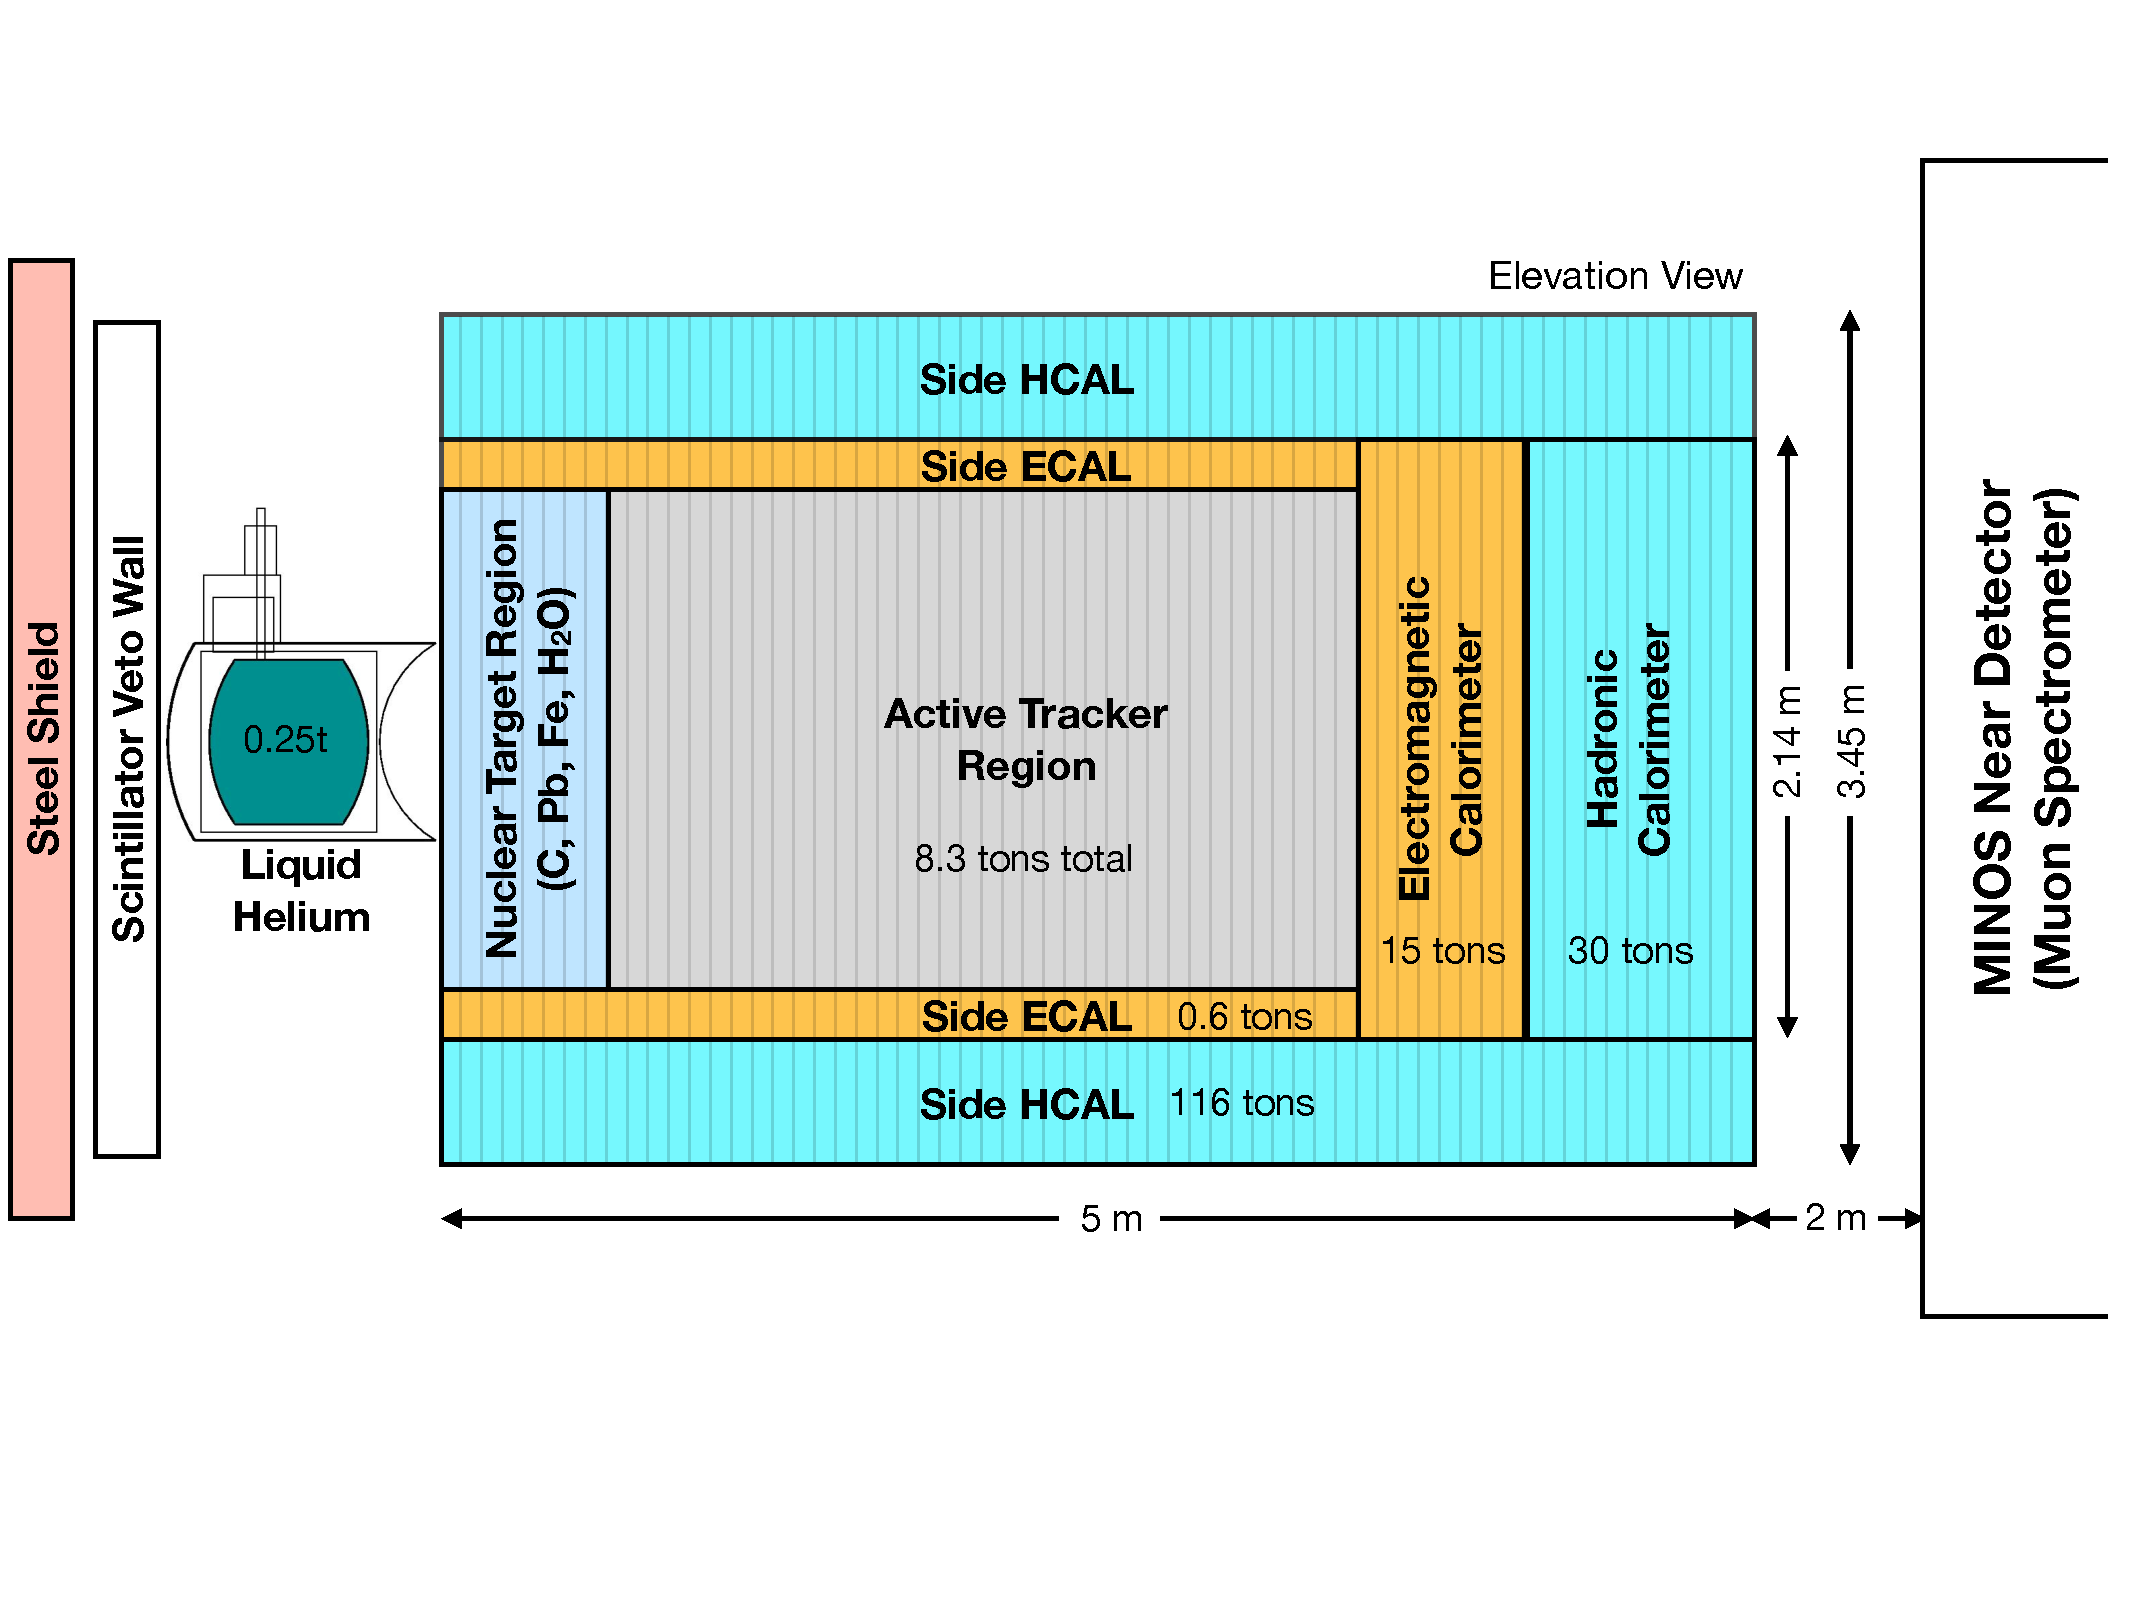
\includegraphics[width=0.60\textwidth]{plots/MINERvA_schematic.pdf}}
  \caption{Schematic of the MINERvA experiment. Reproduced from Figure 1 of Ref.~\cite{minerva-nim}.}
  \label{fig:minerva_detector}
\end{figure}

The central tracking region of MINERvA, and both the electromagnetic and hadronic calorimeters are divided into modules which consist mostly of hexagonal scintillator planes, each made of 127 triangular scintillator bars, arranged in three different orientations (60$^\circ$ rotations between each plane).

There are 62 modules in the fully-active tracker region, each composed of two scintillator layers. A 15 cm border of 0.2 mm thick lead on the downstream end of each module provides electromagetic calorimetry for particles exiting the side of the tracking region. Because the tracker region is fully active, activity around the vertex can be investigated.

The downstream electromagnetic calorimeter is composed of 10 modules, each with two scintillator planes and a 0.2 mm thick lead plate on the downstream end. There are 20 modules in the downstream hadronic calorimeter, each with a single scintillator plane and a 2.54 cm thick hexagonal steel plane. The outer detector consists of a steel frame supporting structure with embedded scintillator planes, as can be seen in Figure~\ref{fig:minerva-module}, which turns the support structure into a hadronic calorimeter. The combination of the downstream and side electromagnetic and hadronic calorimeters allows for containment of most particles produced by vertices within the central tracking region, and allows for particle identification and momentum measurements.

\subsection{Detector physics studies possible with MINERvA components}
